\documentclass[a4paper, 11pt]{article}

\usepackage{graphicx}
\graphicspath{{public/}}

\usepackage{geometry}
\geometry{left=1.5cm, right=1.5cm, top=3cm, bottom=2cm}

\usepackage{array}


\begin{document}

\title{\textbf{Threat modeling deliverables}}
\author{\textit{Qiyang Gu, Zhiyuan Li}}
\date{}
\maketitle


\section*{Step 1: Identify assets}
An asset is defined as a conceptual or concrete property which is of attacker’s importance. They can be termed as threat targets. In our case, the SQLite Database Engine, all the non-null attributes of extracted database are considered as very important assets. 

\begin{table}[htbp]

\centering
\begin{tabular}{| m{1cm} || >{\raggedright}m{4cm} || m{12cm} |}    
\hline
\multicolumn{1}{|c||}{ID} & \multicolumn{1}{c||}{Name} & \multicolumn{1}{c|}{Description} \\
\hline
1 & System & Assets relating to the underlying system. \\
\hline
1.1 & Availability of SQLite Database & The SQLite Database should be available 24 hours a day and can be accessed by all database users, database administrators, and system administrators. \\
\hline
1.2 & Ability to Execute SQL Command as a Database Read User & This is the ability to execute SQL select queries on the database, and thus retrieve any information stored in database. \\
\hline
1.3 & Ability to Execute SQL as a Database Read/Write User & This is the ability to execute SQL command, such as select, insert, and update queries on the database and thus have read and write access to any information stored in database. \\
\hline
2 & Database Engine & Assets relating to the SQLite database engine. \\
\hline
2.1 & Login Session & This is the login session of a user to the Sqlite database. This user could be a normal user, database administrator, or a system administrator. \\
\hline
2.2 & Data Stored in Database & The information is stored in SQLite database in various tables using different attributes, which may include sensitive information such as username, password, email address, banking details. \\
\hline
2.3 & Database Backup & The database backup is a copy of data from database that can be used to reconstruct that data. \\
\hline
2.4 & Transaction Log & It records all transactions and the database modifications made by each transaction. \\
\hline
\end{tabular}
\caption{Assets of SQLite}
\end{table}



\section*{Step 2: Create an architecture overview}
\setcounter{section}{2}
\subsection{Architecture diagram}
% 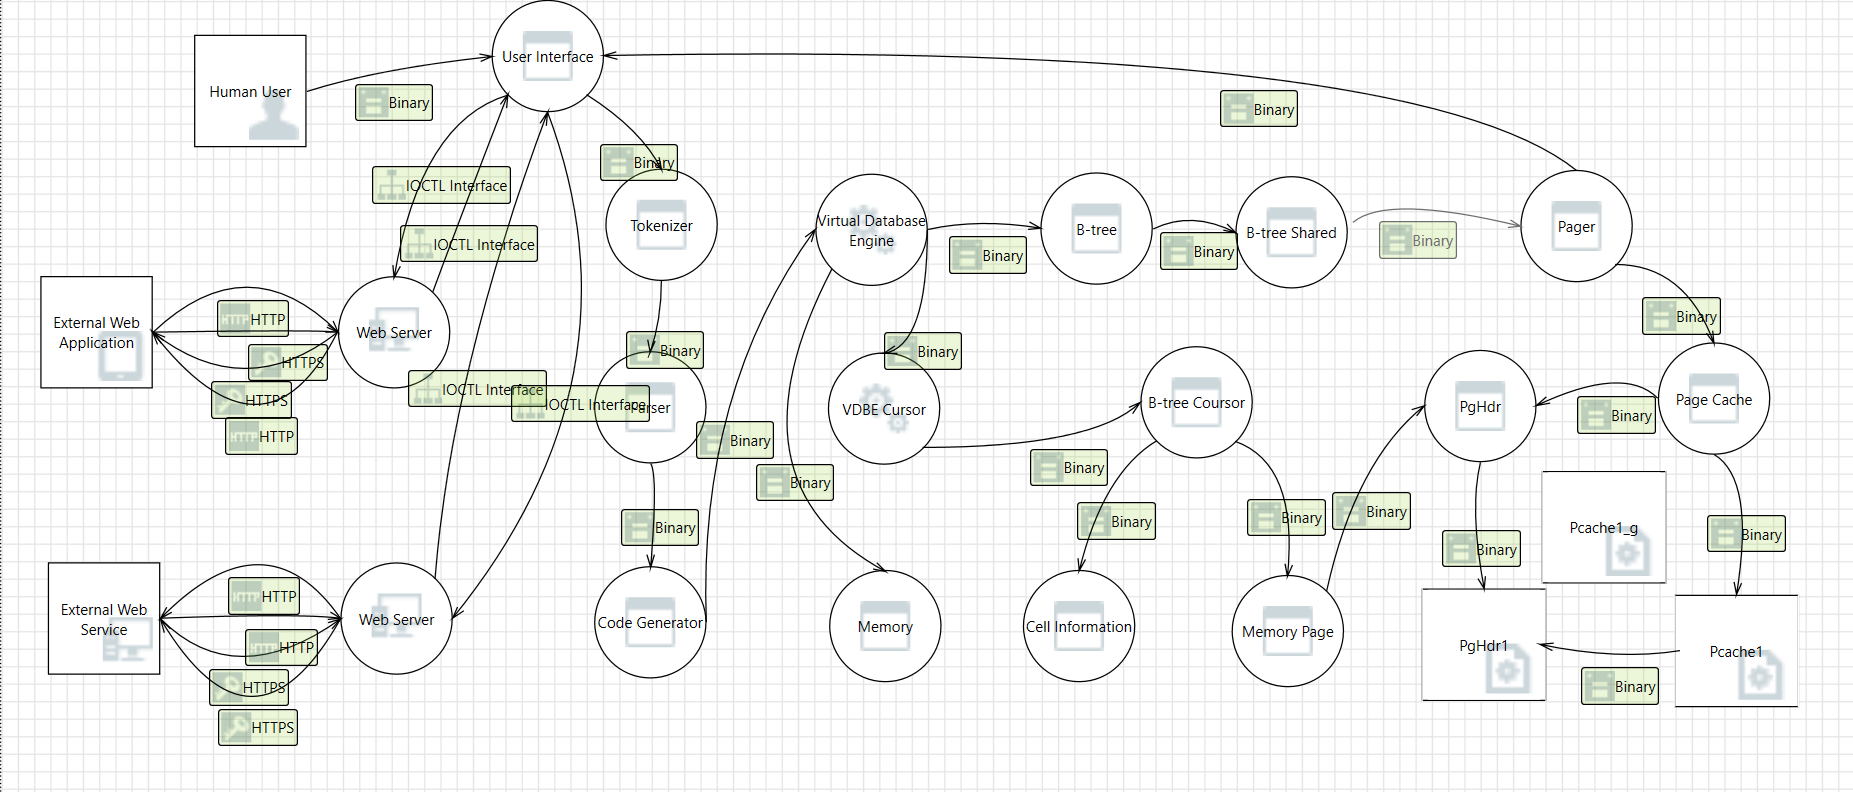
\includegraphics[height=7.7cm]{arch.png}



\section*{Step 3: Decompose the application}


\section*{Step 4: Identify the threats}


\section*{Step 5: Document the threats}


\section*{Step 6: Rate the Threats}


\end{document}